% ============================================================
% Token-Balanced Fine-Tuning Is Not Loss-Balanced
% arXiv version. Every number is computed from results.jsonl.
% Compile: pdflatex, bibtex, pdflatex, pdflatex.
% ============================================================
\documentclass[11pt]{article}
\usepackage[margin=1in]{geometry}
\usepackage[T1]{fontenc}
\usepackage{times}
\usepackage{booktabs}
\usepackage{amsmath}
\usepackage{graphicx}
\usepackage{multirow}
\usepackage{natbib}
\usepackage{url}
\usepackage{xcolor}
\usepackage[colorlinks=true,linkcolor=blue!50!black,citecolor=blue!50!black,urlcolor=blue!50!black]{hyperref}
\emergencystretch=3em

\title{Token-Balanced Fine-Tuning Is Not Loss-Balanced:\\
Pretraining Coverage, Not Scale, Predicts the Gap}

\author{Sagar Singhal\\
Independent Researcher\\
\texttt{ss.sagarsinghal16@gmail.com}}
\date{October 2026}

\begin{document}
\maketitle

\begin{abstract}
Fine-tuning corpora are routinely balanced by token count across topics, on
the assumption that equal exposure produces equal improvement. We show that
this assumption fails, and then identify what determines the size of the
failure. Fine-tuning GPT-2 small, Pythia-160M and Pythia-410M on strictly
token-balanced three-topic mixtures drawn from Wikipedia, arXiv abstracts
and FineWeb-Edu, mathematics attains the largest held-out loss reduction in
27 of 27 runs, leading the runner-up by 3.4 to 12.7 percentage points. The
gap is not a transient of early adaptation: it persists and widens as the
per-topic budget grows from 2M to 16M tokens. Its size is not intrinsic to
topics either, varying jointly with corpus and model (topic $\times$ corpus
$\times$ model interaction, run-level permutation $p<10^{-4}$). Controlled comparisons then separate the candidate causes. Holding the model
fixed, replacing full fine-tuning with LoRA shrinks the margins from
4.1/6.3/7.1\,pp to 1.2/4.9/1.6\,pp, and raising the LoRA rank recovers part
of the gap. Holding parameter count and adapter fixed, replacing Pythia-410M
with Qwen2.5-0.5B shrinks them to 0.0/0.0/0.5\,pp. Neither scale variable
matters: scaling 0.5B $\to$ 1.5B $\to$ 7B within the Qwen family, or
pretraining Pythia-410M for 8B versus 300B tokens, leaves the margin
essentially unchanged. What predicts it is the base model's existing
coverage of each topic. Across five pretraining recipes, the further
mathematics already sits below the other topics in base-model loss, the
smaller the margin fine-tuning produces, in all three corpora (mean
within-corpus Spearman $\rho{=}0.83$, exact stratified permutation
$p{=}0.0013$); the two recipes that emphasize mathematical data show the
smallest margins. We additionally falsify three candidate explanations of
the topic ordering: absolute baseline headroom, lexical overlap, and
token-class composition. We release the corpus-construction pipeline, the per-run results, and the analysis code.
\end{abstract}

\section{Introduction}

When practitioners assemble a corpus for fine-tuning or continued
pretraining, a standard recipe is to balance it by token count: if the goal
is a model that improves evenly across several topics, each topic
contributes an equal number of tokens. The implicit expectation is that
equal exposure yields equal improvement. A substantial line of work on data
mixing optimizes domain proportions for downstream performance
\citep{doremi,doge,regmix}, taking unequal domain value as its starting
point; the prior question of whether \emph{equal} proportions deliver equal
learning has received little direct scrutiny.

\paragraph{Practical takeaway.} Before balancing a fine-tuning mixture by
tokens, measure the base model's loss on each topic. Across the five
pretraining recipes we compare, the further mathematics already sits below
the other topics at baseline, the less extra improvement a balanced mixture
gives it (Section~\ref{sec:decomp}). Where baseline losses are near parity,
a balanced mixture can improve one topic far more than another, by up to
12.7\,pp under full fine-tuning in our experiments. We tested this for
mathematics only; whether it holds for other topics is open.

We measure improvement as held-out relative loss reduction, and we say a
mixture is \emph{loss-balanced} when that quantity is approximately equal
across topics. We deliberately do not call this ``learning'': loss reduction need not translate into task capability, and we do not measure capability here. The
narrower claim is the one our measurements support.

Our first result is that token-balanced mixtures are not loss-balanced.
Across three model families, three corpora and three seeds (27 runs),
mathematics attains the largest relative loss reduction every time, with
margins over the runner-up from 3.4 to 12.7\,pp. Increasing the per-topic
budget eightfold, from 2M to 16M tokens, does not close the gap; on
Wikipedia it grows from 6.1 to 9.9\,pp. The gap also survives a 2.5-fold
change in learning rate.

Our second and more consequential result is that this inequality is a
property of the training regime rather than of the topics. Its size depends
jointly on corpus and model, and controlled comparisons separate the
candidate causes. Replacing full fine-tuning with LoRA on the same model
roughly halves the margins, and a rank sweep shows the margin rising again
with adapter capacity. Replacing that model with a similarly sized model
from a modern pretraining run (Pythia-410M versus Qwen2.5-0.5B, with adapter
and token budget held fixed) removes almost all of what remains. The two
variables most often invoked when a small-model effect is doubted do not
matter: scaling within the Qwen family from 0.5B to 7B changes nothing of
practical size, and neither does pretraining Pythia-410M for 36 times as many tokens.

What does predict the margin is how well the base model already covers
each topic. We measure this directly, as the base model's loss on
mathematical text relative to the other two topics, and compare five
pretraining recipes at a fixed adapter and budget. Within every corpus, the
further mathematics already sits below the others, the smaller the margin
(mean within-corpus $\rho{=}0.83$, exact $p{=}0.0013$). The two recipes that
emphasize mathematical data, Qwen2.5 and SmolLM2, sit at one end; three
general-web recipes sit at the other, regardless of parameter count. More
pretraining on a fixed mixture does not move a model along this axis;
a different mixture does. The inequality a study on an older base model
would find is real, and it shrinks as pretraining mixtures cover the
fine-tuning domain more heavily.

We also ask why mathematics is the advantaged topic when the effect is
present, and report three failures. A cross-corpus transfer matrix shows
that mathematical evaluation text is unusually \emph{receptive}: it improves
when the model is fine-tuned on any other topic drawn from the same corpus
(mean $+6.3\%$, against $-0.4\%$ for computer science and $+0.3\%$ for
physics), while the topic-specific residual is nearly equal across topics
(13.1/11.5/12.3\%). Baseline headroom does not predict this receptivity
($\rho{=}0.00$); n-gram coverage does not (computer-science-to-mathematics
and mathematics-to-computer-science training share identical 8-gram
coverage of 0.4\% yet transfer $+16.1$ versus $+0.2$\,pp); and a per-token
decomposition shows the cross-topic gain is not concentrated in notation
tokens. We report the mechanism as open.

\paragraph{Contributions.}
\begin{itemize}
  \item Token-balanced fine-tuning is not loss-balanced: mathematics ranks
  first in 27/27 runs across three model families, three corpora and three
  seeds, with margins of 3.4--12.7\,pp; the ordering survives an eightfold
  budget increase and a 2.5-fold learning-rate change.
  \item Controlled comparisons decompose the margin. Adapter capacity
  matters (full fine-tuning $\to$ LoRA shrinks it; higher LoRA rank
  partly restores it). Scale does not, whether measured as parameters
  (0.5B--7B within one family) or as pretraining length (8B--300B tokens
  within one model).
  \item Across five pretraining recipes, the base model's existing
  coverage of a topic predicts the margin in every corpus (exact stratified
  permutation $p{=}0.0013$), with math-emphasis recipes producing the
  smallest margins.
  \item We falsify three explanations for the topic ordering (absolute
  baseline headroom, lexical overlap, and token-class composition) and
  characterize the phenomenon as evaluation-set receptivity, which we leave
  unexplained.
  \item We release the pipeline that builds a nine-cell corpus with document-level splitting and explicit 13-gram decontamination against the evaluation sets, together with the per-run results and the analysis code.
\end{itemize}

\section{Related Work}
\label{sec:related}

\paragraph{Data mixing and domain reweighting.}
A growing body of work optimizes the proportions of training domains for
downstream performance: DoReMi learns domain weights with a small proxy
model \citep{doremi}, DoGE reweights domains by estimated generalization
contribution \citep{doge}, and RegMix casts mixture selection as regression
over small-scale proxy runs \citep{regmix}. These methods presuppose that
domains differ in learning value and search for non-uniform mixtures; our
question is prior to theirs: whether the \emph{uniform} mixture, widely used
as a default, even delivers uniform improvement. We find it does not under
some training regimes and essentially does under others, and we characterize
which. Our setting is a balanced multi-domain instance of continued
pretraining, whose single-domain benefits are well established
\citep{gururangan2020dont}.

\paragraph{Text statistics as proxies for data value.}
Entropy- and diversity-based statistics have been proposed as inexpensive
proxies for a domain's training value \citep{bimix}. Our results complicate
this picture in two ways: within our data, neither lexical overlap nor
baseline perplexity predicts which evaluation sets benefit from out-of-topic
training, and the quantity such proxies would need to predict is itself
regime-dependent.

\paragraph{Parameter-efficient adaptation.}
LoRA \citep{lora} and its quantized variant QLoRA \citep{qlora} are now
standard for adapting large models under limited memory. They are usually
evaluated on whether they match full fine-tuning in aggregate. We use the
comparison differently: holding the model and data fixed, the adapter
changes how \emph{unevenly} a balanced mixture is absorbed, which is a
property aggregate comparisons do not surface.

\paragraph{Reliability of analysis findings.}
Single-dataset analyses of neural models can suggest regularities that fail
to generalize: \citet{bolukbasi2021illusion} document an ``interpretability
illusion'' in which neuron-level conclusions drawn from one corpus do not
hold on others. Our study contributes a training-dynamics instance of the
same concern, and extends it: the effect we measure is stable across corpora
in direction but its magnitude is contingent on the base model, so a claim
established on one model generation may not describe the next.

\section{Experimental Setup}
\label{sec:setup}

\paragraph{Corpora.}
We build nine corpus--topic cells: three topics (mathematics, computer
science, physics) drawn from three sources. Wikipedia articles are collected
by category traversal from hand-selected seed categories per topic (depth
limited; administrative, biographical and list categories excluded), with
cleaned article prose retained. An article reachable from more than one
topic's traversal is dropped from all of them, so the three Wikipedia topics
are disjoint by construction; this strict rule is why the mathematics cell
is the smallest. arXiv abstracts\footnote{From the public
\texttt{gfissore/arxiv-abstracts-2021} dataset on the Hugging Face Hub.} are
assigned by \emph{primary} category prefix (\texttt{math.*}; \texttt{cs.*}; \texttt{physics.*},
\texttt{astro-ph}, \texttt{cond-mat}, \texttt{hep-*}, \texttt{gr-qc},
\texttt{quant-ph}, \texttt{nucl-*}), with any abstract cross-listed into a
second target topic discarded. FineWeb-Edu \citep{penedo2024fineweb} documents
are selected by a per-topic keyword score and then verified by a zero-shot NLI classifier,
keeping only documents whose top label matches the keyword assignment with
confidence $\geq 0.6$.

\paragraph{Splitting and decontamination.}
Exact duplicates are removed globally. Every document is then assigned
wholly to the training or evaluation partition by a deterministic hash of
its normalized text (1 in 20 to evaluation), before tokenization, so the
evaluation set is fixed across seeds, models and budgets. We additionally
remove from the training partition any document that shares at least ten
13-grams, or at least 10\% of its 13-grams, with the evaluation pool of its
cell. This removed at most 125 documents from any cell; the largest proportional
removal was in FineWeb-Edu mathematics, at about 4\% of its training
documents. The 13-gram criterion follows the contamination analysis of
\citet{brown2020gpt3}. The check matters: before decontamination, 2.73\% of
FineWeb-Edu mathematics evaluation documents had at least half their
13-grams present in a 2M-token sample of the training pool (worksheet-style
pages that recur across the web), and the FineWeb-Edu margins fell by
0.5--2.1\,pp after removal without changing any ordering. Every other cell,
on and off the diagonal, was at 0.00\%.

\paragraph{Models and training.}
The full-fine-tuning experiments use GPT-2 small (124M)
\citep{radford2019language}, Pythia-160M and Pythia-410M
\citep{biderman2023pythia}. The parameter-efficient experiments use
Pythia-410M, Qwen2.5-0.5B, Qwen2.5-1.5B and Qwen2.5-7B \citep{qwen25} with
LoRA \citep{lora} at rank 16, $\alpha{=}32$, applied to all attention and
MLP projections; the 7B model additionally uses 4-bit NF4 quantized base
weights \citep{qlora}. A rank control repeats the Pythia-410M LoRA runs at
ranks 4 and 64, with $\alpha{=}2r$ so the adapter scale is unchanged. A
pretraining-length control fine-tunes Pythia-410M from four intermediate
checkpoints (steps 4k, 16k, 36k and 72k, roughly 8B to 151B tokens) as well
as the final one (300B), all of which share architecture, tokenizer and data
order. A cross-family panel adds three base models with documented
pretraining mixtures at the same LoRA setting: TinyLlama-1.1B, trained on 3T
tokens of SlimPajama and Starcoderdata at roughly 7:3 natural language to
code \citep{zhang2024tinyllama}; OLMo-1B, trained on Dolma
\citep{groeneveld2024olmo,soldaini2024dolma}; and SmolLM2-360M, trained on 4T
tokens of a mixture that includes FineWeb-Edu and dedicated curated
mathematics datasets \citep{allal2025smollm2}. Mixtures are strictly token-balanced, tokenized with
each model's native tokenizer, concatenated into 512-token blocks, pooled
and shuffled. We train one pass with AdamW, batch size 8, weight decay 0.01,
100 warmup steps then linear decay, gradient clipping at 1.0. Full
fine-tuning uses $5\times10^{-5}$ (with a $2\times10^{-5}$ control,
Section~\ref{sec:robust}); LoRA uses $1\times10^{-4}$, and we never compare
across learning rates without saying so. Every configuration is replicated
over three seeds. GPT-2 runs use bf16 autocast; Pythia diverged under
autocast with fp32 weights and is run in fp32 throughout.

\paragraph{Evaluation.}
For each cell we compute perplexity on its fixed held-out blocks (200K
tokens) before and after fine-tuning, and report relative reduction,
$100\times(\mathrm{ppl}_{\text{base}}-\mathrm{ppl}_{\text{ft}})/\mathrm{ppl}_{\text{base}}$.
Percentages denote relative reductions; pp denotes a difference between two
such reductions. Every fine-tuned model is evaluated on all nine cells, not
only its own.

\paragraph{Statistics.}
The experimental unit is one trained model. Topic is within-run; corpus,
model, budget, adapter and learning rate are between-run. We report
split-plot $F$ tests for the interactions of interest and, because seed
variance on fixed evaluation sets is very small and inflates $F$, we treat
run-level permutation tests as primary: group labels are permuted across
runs and the $F$ statistic recomputed, exactly where the number of distinct
relabelings is small enough (1,680 for one model across three corpora) and
by $10^4$ Monte Carlo draws otherwise, where $p<10^{-4}$ is the smallest value
the procedure can return. For the cross-family panel, where the
unit is a base model and each corpus contributes one point per family, we
test the within-corpus Spearman correlation between baseline coverage and
margin with an exact stratified permutation test: margins are permuted only
within each corpus, across all $5!\times5!\times4!=345{,}600$ relabelings,
so differences between corpora cannot produce the effect. We report raw
margins and seed ranges throughout and do not report standardized effect
sizes at $n{=}3$.

\section{Token-Balanced Is Not Loss-Balanced}
\label{sec:main}

Figure~\ref{fig:ordering} and Table~\ref{tab:e1} report the three full-fine-tuning models on all three
corpora at 2M tokens per topic. Mathematics attains the largest relative
loss reduction in all 27 runs. Margins over the runner-up range from 3.4\,pp
(Pythia-160M on Wikipedia) to 12.7\,pp (GPT-2 on arXiv). Seed spread is at
most 0.6\,pp and usually below 0.3\,pp.

\begin{table}[t]
\centering
\caption{Relative held-out loss reduction (\%) under token-balanced
three-topic fine-tuning, 2M tokens per topic, mean $\pm$ s.d.\ over three
seeds. Margin is mathematics minus the runner-up.}
\label{tab:e1}
\small
\begin{tabular}{llrrrrc}
\toprule
Model & Corpus & Math & CS & Physics & Margin (pp) & Math first \\
\midrule
GPT-2 small & Wikipedia   & 11.5$\pm$0.2 & 5.1$\pm$0.1 & 5.4$\pm$0.1 & 6.1 & 3/3 \\
GPT-2 small & arXiv       & 40.5$\pm$0.1 & 24.3$\pm$0.1 & 27.8$\pm$0.0 & 12.7 & 3/3 \\
GPT-2 small & FineWeb-Edu & 12.8$\pm$0.1 & 8.0$\pm$0.1 & 9.2$\pm$0.1 & 3.6 & 3/3 \\
Pythia-160M & Wikipedia   & 8.3$\pm$0.2 & 4.8$\pm$0.3 & 3.2$\pm$0.2 & 3.4 & 3/3 \\
Pythia-160M & arXiv       & 23.0$\pm$0.1 & 16.3$\pm$0.1 & 14.5$\pm$0.1 & 6.7 & 3/3 \\
Pythia-160M & FineWeb-Edu & 11.4$\pm$0.1 & 4.3$\pm$0.1 & 4.1$\pm$0.1 & 7.1 & 3/3 \\
Pythia-410M & Wikipedia   & 1.2$\pm$0.6 & $-$2.9$\pm$0.4 & $-$4.0$\pm$0.2 & 4.1 & 3/3 \\
Pythia-410M & arXiv       & 14.9$\pm$0.1 & 8.6$\pm$0.1 & 6.0$\pm$0.1 & 6.3 & 3/3 \\
Pythia-410M & FineWeb-Edu & 3.3$\pm$0.1 & $-$3.8$\pm$0.2 & $-$3.9$\pm$0.2 & 7.1 & 3/3 \\
\bottomrule
\end{tabular}
\end{table}

\begin{figure}[t]
\centering
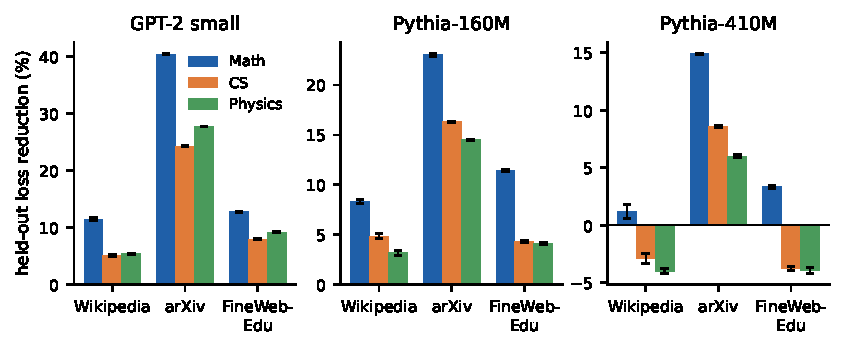
\includegraphics[width=\textwidth]{fig1_ordering.pdf}
\caption{Relative held-out loss reduction by topic, corpus and model, at 2M
tokens per topic under full fine-tuning. Error bars are one standard
deviation over three seeds. Mathematics leads in all 27 runs, but the size
of its lead and the identity of the runner-up both change with the model.
Note the differing $y$ scales.}
\label{fig:ordering}
\end{figure}

The margin is not intrinsic to the topics. A split-plot analysis over all 27
runs gives a topic $\times$ corpus $\times$ model interaction of
$F(8,36)=352.5$, run-level permutation $p<10^{-4}$; the two-way terms are
$F(4,36)=737.3$ for topic $\times$ corpus and $F(4,36)=365.3$ for topic
$\times$ model, both with permutation $p<10^{-4}$. For GPT-2 alone the
topic $\times$ corpus interaction has exact permutation $p=0.001$ over all
1,680 relabelings. Concretely, which corpus
produces the largest inequality depends on the model: for GPT-2 it is arXiv
(12.7\,pp, against 6.1 and 3.6), while for both Pythia models it is
FineWeb-Edu (7.1\,pp, against 3.4/4.1 and 6.7/6.3). Mean-centering each
run's three gains on that run's own mean removes the corpus-level shift in
overall improvement; mathematics then sits between $+2.8$ and $+9.6$\,pp
above its run mean in every one of the nine model--corpus cells, with seed
spread at most 0.3\,pp. The runner-up also changes: GPT-2 places physics second everywhere, Pythia-160M places computer
science second on two corpora of three. Restricted to a single model and a
single corpus, one would report a clean fact about topics; the fact does not
survive changing either.

\section{Robustness: Budget and Learning Rate}
\label{sec:robust}

Two objections apply to any result of this kind at this scale. The first is
that 2M tokens is too small a perturbation, so the measurement captures
early surface adaptation rather than anything durable. Table~\ref{tab:e3} and Figure~\ref{fig:budget}
answer it: raising the budget to 8M and 16M tokens per topic leaves
mathematics first at every budget and, on Wikipedia, widens the margin from
6.1 to 9.9\,pp. The topic $\times$ budget interaction is significant
($F(4,24)=603.2$, permutation $p<10^{-4}$) because the gap changes size,
growing on Wikipedia and shrinking slightly on arXiv from 12.7 to
11.6\,pp, but it does not change sign.

\begin{table}[t]
\centering
\caption{Budget scaling, GPT-2 small, three-topic mixture. Relative
reduction (\%), mean over three seeds.}
\label{tab:e3}
\small
\begin{tabular}{llrrrr}
\toprule
Corpus & Tokens/topic & Math & CS & Physics & Margin (pp) \\
\midrule
Wikipedia & 2M  & 11.5 & 5.1 & 5.4 & 6.1 \\
Wikipedia & 8M  & 18.0 & 8.2 & 9.4 & 8.6 \\
Wikipedia & 16M & 21.7 & 10.0 & 11.8 & 9.9 \\
arXiv     & 2M  & 40.5 & 24.3 & 27.8 & 12.7 \\
arXiv     & 8M  & 51.9 & 33.8 & 39.5 & 12.3 \\
arXiv     & 16M & 56.8 & 38.5 & 45.3 & 11.6 \\
\bottomrule
\end{tabular}
\end{table}

\begin{figure}[t]
\centering
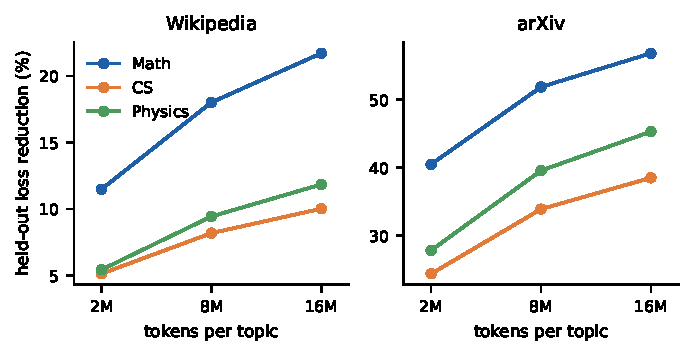
\includegraphics[width=0.8\textwidth]{fig2_budget.pdf}
\caption{Budget scaling, GPT-2 small. The ordering is unchanged from 2M to
16M tokens per topic and the mathematics margin does not close; on Wikipedia
it widens from 6.1 to 9.9\,pp.}
\label{fig:budget}
\end{figure}

The second objection concerns the learning rate, since Pythia-410M shows
negative reductions for computer science and physics on two corpora in
Table~\ref{tab:e1}; there, mathematics is the only topic that does not get
worse. Repeating those nine runs at $2\times10^{-5}$ makes all three topics
positive on all three corpora (Wikipedia 6.4/3.2/2.7, arXiv 17.7/11.5/10.5,
FineWeb-Edu 7.2/2.0/2.3) while leaving mathematics first in 18 of 18 runs
across both rates (Figure~\ref{fig:lr}). The topic $\times$ learning-rate interaction is
significant ($F(2,24)=132.4$, permutation $p<10^{-4}$): the rate sets how
large the gains are, not which topic leads.

\begin{figure}[t]
\centering
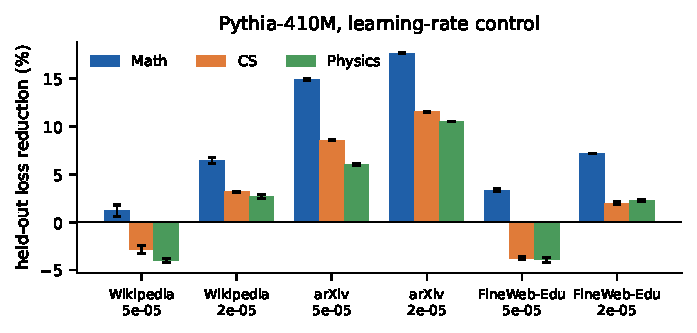
\includegraphics[width=0.8\textwidth]{fig5_lr.pdf}
\caption{Learning-rate control on Pythia-410M. The lower rate makes every
topic improve on every corpus; mathematics leads at both rates.}
\label{fig:lr}
\end{figure}

\section{What Determines the Size of the Inequality}
\label{sec:decomp}

Table~\ref{tab:decomp} and Figure~\ref{fig:decomp} give the three main
comparisons, each changing one factor. Two further controls (adapter rank
and pretraining length, Table~\ref{tab:controls}) and a five-recipe panel
(Table~\ref{tab:panel}, Figure~\ref{fig:panel}) then test what the family
difference tracks.

\begin{table}[t]
\centering
\caption{Three controlled comparisons. Each row block changes exactly one
factor. Margins are the leading topic minus the runner-up, in pp, mean over
three seeds; the leading topic is mathematics except for Qwen2.5-1.5B and
Qwen2.5-7B on Wikipedia, where it is computer science. The 7B model uses
4-bit base weights.}
\label{tab:decomp}
\small
\begin{tabular}{llrrrl}
\toprule
Comparison & Condition & Wiki & arXiv & Edu & Test \\
\midrule
\multirow{2}{*}{Adapter (Pythia-410M)}
 & full fine-tuning & 4.1 & 6.3 & 7.1 & \multirow{2}{*}{$F(2,24)=926.9$, $p_{\text{perm}}<10^{-4}$} \\
 & LoRA             & 1.2 & 4.9 & 1.6 & \\
\midrule
\multirow{2}{*}{Pretraining ($\approx$0.5B, LoRA)}
 & Pythia-410M (300B) & 1.2 & 4.9 & 1.6 & \multirow{2}{*}{$F(2,24)=3121.6$, $p_{\text{perm}}<10^{-4}$} \\
 & Qwen2.5-0.5B (18T) & 0.0 & 0.0 & 0.5 & \\
\midrule
\multirow{3}{*}{Scale (Qwen, LoRA)}
 & 0.5B & 0.0 & 0.0 & 0.5 & \multirow{3}{*}{$F(4,36)=62.9$, $p_{\text{perm}}<10^{-4}$} \\
 & 1.5B & 0.1 & 0.2 & 0.4 & \\
 & 7B   & 0.6 & 0.9 & 0.3 & \\
\bottomrule
\end{tabular}
\end{table}

\begin{figure}[t]
\centering
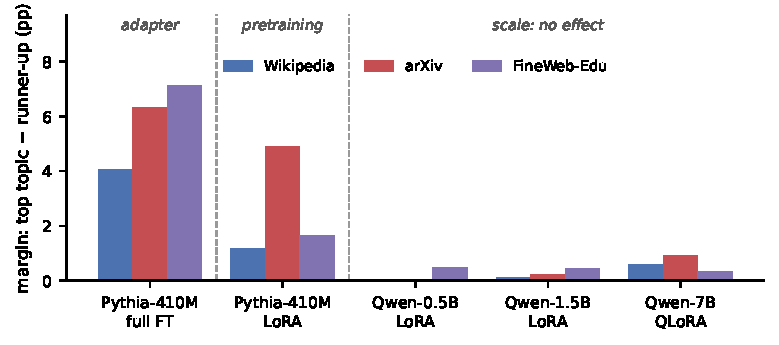
\includegraphics[width=0.9\textwidth]{fig3_decomposition.pdf}
\caption{The margin between the leading topic and the runner-up under five
training regimes, all at 2M tokens per topic. Changing the adapter (first
gap) and changing the pretraining run at fixed parameter count (second gap)
each remove a large part of the inequality. Scaling within the Qwen family,
with pretraining and adapter held fixed, does not.}
\label{fig:decomp}
\end{figure}

\paragraph{Adapter.} Holding the model, data, corpora and budget fixed and
replacing full fine-tuning with LoRA reduces every margin, by between a
fifth (arXiv) and four fifths (FineWeb-Edu). Mathematics still ranks first
in 9 of 9 LoRA runs, so the adapter compresses the inequality without
removing it. The compression tracks adapter capacity rather than being a
property of one setting (Table~\ref{tab:controls}): ranks 4 and 16 give
nearly identical margins, rank 64 gives larger ones on every corpus
(1.9/5.8/2.8\,pp), and full fine-tuning the largest. Mathematics ranks
first in all 27 runs across the three ranks.

\paragraph{Pretraining coverage.} Holding parameter count in the same
bracket and the adapter fixed, and changing only which model is adapted,
removes almost all of what remains: from 1.2/4.9/1.6 to 0.0/0.0/0.5. On
arXiv, mathematics and physics tie at 8.6\% and mathematics ranks first in
only 1 of 3 runs. In proportional terms this is the largest of the three effects: it removes roughly 90\% of the remaining margin, against roughly 57\% for the adapter switch.

\paragraph{Scale.} Holding pretraining data and adapter fixed and scaling
0.5B $\to$ 1.5B $\to$ 7B, the margins are 0.0/0.0/0.5, 0.1/0.2/0.4 and
0.6/0.9/0.3. The interaction is nominally significant but the effect is
negligible in size and non-monotone; if anything the margin drifts slightly
upward with scale. We report this as no practically meaningful scale effect,
and note that the significance is an artifact of near-zero seed variance.
The objection usually raised against small-model findings, that the effect
would go away at 7B, is within this family false; what makes it
appear true across families is pretraining, not size.

\paragraph{Pretraining length.} A second objection is that small models show
the effect because they are undertrained. Pythia-410M's intermediate
checkpoints test this directly, since they differ only in how many tokens
the model has seen. The sweep runs from 8B tokens, close to the
compute-optimal ratio of about 20 tokens per parameter
\citep{hoffmann2022chinchilla}, to 300B, roughly 36 times more. Nothing
moves (Table~\ref{tab:controls}). Mathematics ranks first in all 45 runs.
The margin stays within 3.0--4.1\,pp on Wikipedia, 5.4--6.3 on arXiv and
5.4--8.0 on FineWeb-Edu, with no monotone trend, and the base model's
coverage gap on mathematics (defined below) moves by less than 2 points on
every corpus. More pretraining on a fixed mixture changes neither quantity.

\begin{table}[t]
\centering
\caption{Two further controls on Pythia-410M, 2M tokens per topic, three
seeds. Margin is mathematics minus the runner-up, in pp; mathematics ranks
first in every run shown. Top: LoRA rank at the final checkpoint
($\alpha{=}2r$). Bottom: full fine-tuning from intermediate pretraining
checkpoints. Coverage gap is defined in the text; it is shown for the
checkpoint sweep, where it would have to change for pretraining length to
matter.}
\label{tab:controls}
\small
\begin{tabular}{llrrrrrr}
\toprule
 & & \multicolumn{2}{c}{Wikipedia} & \multicolumn{2}{c}{arXiv} & \multicolumn{2}{c}{FineWeb-Edu} \\
 & Condition & gap & margin & gap & margin & gap & margin \\
\midrule
\multirow{4}{*}{Adapter} & LoRA $r{=}4$  & & 1.2 & & 5.1 & & 1.5 \\
 & LoRA $r{=}16$ & & 1.2 & & 4.9 & & 1.6 \\
 & LoRA $r{=}64$ & & 1.9 & & 5.8 & & 2.8 \\
 & full fine-tuning & & 4.1 & & 6.3 & & 7.1 \\
\midrule
\multirow{5}{*}{Pretraining} & 8B tokens   & $-11.9$ & 3.7 & $-22.1$ & 5.7 & $-0.5$ & 8.0 \\
 & 34B  & $-12.1$ & 3.0 & $-21.0$ & 5.7 & $+0.1$ & 6.2 \\
 & 75B  & $-11.4$ & 3.4 & $-20.7$ & 6.0 & $+0.4$ & 5.4 \\
 & 151B & $-11.8$ & 3.0 & $-20.7$ & 5.4 & $+0.1$ & 5.7 \\
 & 300B (final) & $-11.8$ & 4.1 & $-20.5$ & 6.3 & $+0.5$ & 7.1 \\
\bottomrule
\end{tabular}
\end{table}

\paragraph{Coverage across pretraining recipes.} If neither size nor length
explains the difference between Pythia and Qwen, what does? We define a base
model's \emph{coverage gap} on a corpus as its baseline loss on
mathematical text relative to the other two topics:
$100\times(\mathrm{ppl}_{\text{math}}-\bar{\mathrm{ppl}}_{\text{other}})/\bar{\mathrm{ppl}}_{\text{other}}$,
where $\bar{\mathrm{ppl}}_{\text{other}}$ is the mean of the computer-science
and physics perplexities. A negative gap means the base model already models
mathematics better than the other topics. We then compare five pretraining
recipes at a fixed LoRA setting (Table~\ref{tab:panel}).

Within every corpus, the more negative the coverage gap, the smaller the
margin (Figure~\ref{fig:panel}). The within-corpus Spearman correlations
are $+1.0$ on Wikipedia (a perfect ordering of the five families), $+0.7$
on arXiv and $+0.8$ on FineWeb-Edu; the mean, $0.83$, has exact stratified
permutation $p{=}0.0013$. The recipes also group as their documented
mixtures suggest. Qwen2.5 and SmolLM2, whose pretraining emphasizes
mathematical data \citep{qwen25,allal2025smollm2}, have the most negative
gaps and the smallest margins (0.0--1.0\,pp); Pythia, TinyLlama and OLMo,
trained on general web, code and scholarly mixtures, have less negative gaps
(between $-12.0$ and $-2.8$ on Wikipedia, and within 2.5 points of zero on
FineWeb-Edu) and margins of 1.2--4.9\,pp. The grouping cuts
across parameter count: SmolLM2-360M is smaller than Pythia-410M and behaves
like Qwen, while TinyLlama-1.1B and OLMo-1B are more than twice the size
of Qwen2.5-0.5B and behave like Pythia. Consistently, within the Qwen family
the residual ordering follows baseline perplexity: on Wikipedia, computer
science has the highest baseline and the largest gain.

Combined with the pretraining-length control, the picture is that a
token-balanced mixture can only redistribute what the base model has not
already absorbed. Training longer on the same mixture does not change what
has been absorbed relative to other topics; training on a different mixture
does. This is correlational across families, which differ in architecture
and tokenizer as well as data, but those differences vary across the panel
while the relationship with coverage holds in every corpus.

\begin{table}[t]
\centering
\caption{Five pretraining recipes at a fixed LoRA setting (rank 16, 2M
tokens per topic, three seeds). Gap: base-model coverage gap on
mathematics, in \%. Margin: mathematics minus the runner-up, in pp.
$^\dagger$SmolLM2 was pretrained on FineWeb-Edu, so its FineWeb-Edu cell is
likely contaminated at the pretraining level and is excluded from the
correlation.}
\label{tab:panel}
\small
\setlength{\tabcolsep}{4pt}
\begin{tabular}{llrrrrrr}
\toprule
 & & \multicolumn{2}{c}{Wikipedia} & \multicolumn{2}{c}{arXiv} & \multicolumn{2}{c}{FineWeb-Edu} \\
Base model & Pretraining & gap & margin & gap & margin & gap & margin \\
\midrule
Qwen2.5-0.5B   & 18T, math emphasis    & $-24.9$ & 0.0 & $-36.1$ & 0.0 & $-21.9$ & 0.5 \\
SmolLM2-360M   & 4T, incl.\ math data  & $-19.0$ & 0.3 & $-27.1$ & 1.0 & $-15.3^\dagger$ & 0.5$^\dagger$ \\
Pythia-410M    & Pile, 300B            & $-12.0$ & 1.2 & $-20.6$ & 4.9 & $+0.6$  & 1.6 \\
TinyLlama-1.1B & SlimPajama+code, 3T   & $-4.9$  & 1.5 & $-8.5$  & 3.8 & $-0.2$  & 1.2 \\
OLMo-1B        & Dolma                 & $-2.8$  & 1.6 & $-7.9$  & 3.8 & $-2.5$  & 1.3 \\
\bottomrule
\end{tabular}
\end{table}

\begin{figure}[t]
\centering
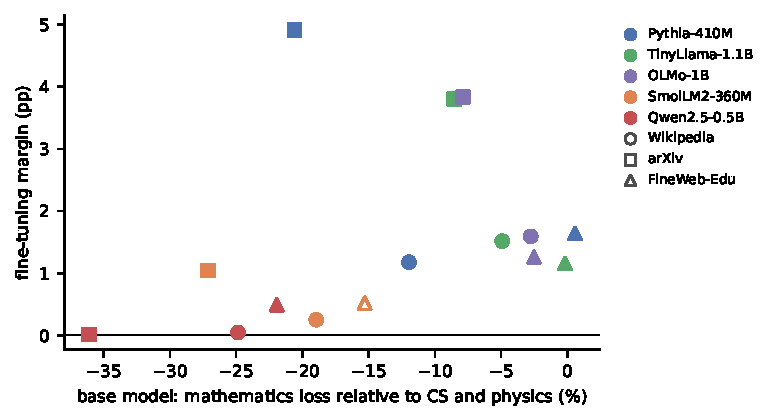
\includegraphics[width=0.8\textwidth]{fig6_panel.pdf}
\caption{Base-model coverage gap on mathematics against the fine-tuning
margin, for five pretraining recipes on three corpora (LoRA rank 16, 2M
tokens per topic). Within each corpus (marker shape), the further
mathematics already sits below the other topics, the smaller the margin.
The hollow marker is SmolLM2 on FineWeb-Edu, excluded as likely
contaminated.}
\label{fig:panel}
\end{figure}

\section{Why Mathematics? Three Explanations That Fail}
\label{sec:why}

The above says when the inequality is large. It does not say why
mathematics is the advantaged topic when it is. We fine-tuned GPT-2 on each
single corpus--topic cell in isolation (2M tokens, three seeds) and
evaluated every resulting model on all nine evaluation sets, giving the
$9\times9$ transfer matrix in Figure~\ref{fig:matrix}.

\begin{figure}[t]
\centering
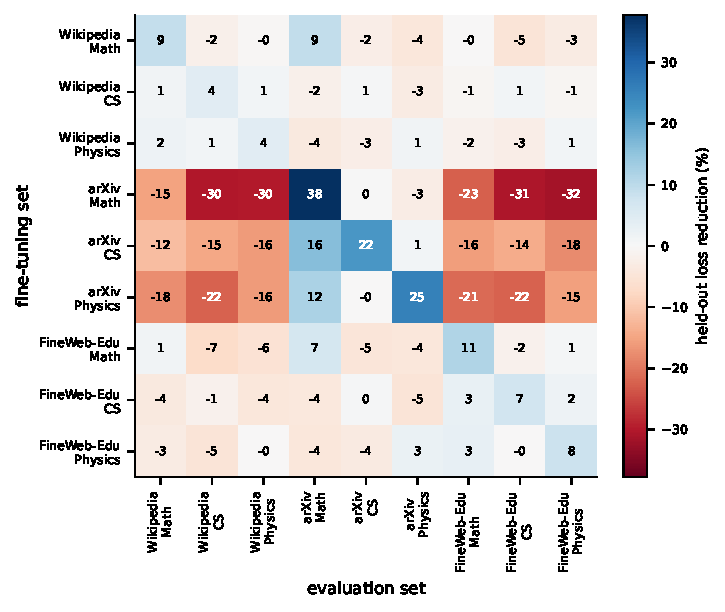
\includegraphics[width=0.72\textwidth]{fig4_matrix.pdf}
\caption{Transfer matrix: GPT-2 fine-tuned on one corpus--topic cell (rows)
and evaluated on all nine (columns), mean over three seeds. The arXiv
mathematics column is the only off-diagonal column with large positive
entries: it gains from computer-science and physics training, while the
reverse directions do not.}
\label{fig:matrix}
\end{figure}

Decomposing each evaluation set's in-cell gain into what other topics of its
own corpus deliver (\emph{receptivity}) and the remainder
(\emph{residual}), mathematics is an outlier in the first and unremarkable
in the second. Mean receptivity is $+6.3\%$ for mathematics, $-0.4\%$ for
computer science and $+0.3\%$ for physics; mean residual is 13.1, 11.5 and
12.3\%. Mathematical evaluation text improves when the model adapts to its
corpus at all, whatever the topic of the adaptation data; the other two
topics do not. The effect is concentrated on arXiv, where fine-tuning on
computer-science abstracts improves mathematics evaluation by $+16.1$\,pp
and fine-tuning on physics abstracts by $+12.1$\,pp, while the reverse
directions give $+0.2$ and $-2.9$\,pp.

Three explanations for this asymmetry fail.

\paragraph{Baseline headroom.} Across the nine evaluation sets, baseline
perplexity correlates with in-cell gain ($\rho{=}0.70$, $p{=}0.036$) but not
at all with receptivity ($\rho{=}0.00$). This is a different quantity from
the coverage gap of Section~\ref{sec:decomp}, and the two results do not
conflict. Here we ask whether an evaluation set's \emph{absolute}
perplexity, within one base model, predicts how much it gains from other
topics; it does not. There we ask whether mathematics' loss
\emph{relative to the other topics}, compared \emph{across} base models,
predicts the margin; it does. Mathematics has the highest baseline perplexity on only one corpus
(FineWeb-Edu, by 0.8 over the other two), and on arXiv it has the lowest
(41.4 against 42.0 and 47.5), yet it is the most receptive on all three.

\paragraph{Lexical overlap.} If mathematical language were a shared
substrate of scientific writing, mathematics evaluation text would share
more $n$-grams with the other topics' training text than the reverse. It
does not. On arXiv, computer-science training covers 0.4\% of the
mathematics evaluation set's 8-grams and mathematics training covers 0.4\%
of the computer-science set's, yet the transfer is $+16.1$ versus $+0.2$\,pp.
Across the 18 within-corpus off-diagonal pairs, coverage and transfer are
uncorrelated ($\rho{=}0.28$, $p{=}0.27$).

\paragraph{Token-class composition.} Retraining each single-topic GPT-2
model once (seed 0) and saving per-token losses, we split each gain over
token classes (digits, symbols,
single characters, short words, longer words). If cross-topic transfer
worked by reshaping the model's distribution over mathematical notation, the
cross-topic gain on arXiv mathematics would concentrate in digit, symbol and
single-character tokens relative to the in-cell gain. Under computer-science
training, symbol tokens do retain a larger share of their in-cell gain than
words (54\% against 38\%). But single-character tokens fall from 5.7\% of
the total gain in-cell to 3.7\% and 2.8\% under computer-science and physics
training, digit tokens contribute essentially nothing, and ordinary words
still carry 34--42\% of the cross-topic gain. The transfer is broad-spectrum, not
notational.

We therefore report receptivity as a measured property without a mechanism.
It is stable across seeds, present on all three corpora, and unexplained by
the three natural candidates.

\section{Discussion}

The practical reading is a decision rule. If you are fully fine-tuning a
model whose pretraining predates the current generation, or one whose
pretraining mixture does not cover your target domain well, a token-balanced
corpus will not give you balanced loss reduction, and the imbalance can
exceed 10\,pp. If instead the base model's pretraining already covers your target domain heavily, as Qwen2.5 and SmolLM2 do for mathematics, then under LoRA token balance is very nearly loss balance (margins of about 1\,pp or less here) and the effort of reweighting buys little. Neither parameter count nor pretraining length is the variable to reason
about. The base model's relative coverage of your topics is, and it is cheap
to measure: evaluate the base model's per-topic loss before fine-tuning. On our evidence, a topic that already sits well below the others will gain least from a balanced mixture, relative to them, and one near parity will gain most; we tested this for mathematics only. Adapter capacity
then scales how much of that asymmetry is realized.

The methodological reading is less comfortable. The effect reported here at
small scale is real, large and replicable, and on our evidence it shrinks as pretraining covers the domain more heavily rather than being refuted. A study run on GPT-2 in 2021
would have found it and generalized; a study run on Qwen2.5 in 2026 would
find almost nothing and conclude it never existed. Both would be reporting
correctly on their own setting. Claims about per-domain learnability are
contingent on a base model's coverage in a way that is rarely stated. We
suggest reporting the base model's per-topic loss alongside any such claim,
since on our evidence it predicts the result better than model size does.

\section*{Limitations}

Our largest model is 7B and our largest budget is 16M tokens per topic;
neither reaches the scale of production continued-pretraining runs, and we
cannot exclude that a different regime appears beyond them. The 7B
comparison uses 4-bit quantized base weights, which the 0.5B and 1.5B
comparisons do not, so the scale ladder confounds quantization with size at
its top point; the 0.5B-to-1.5B step, which is unconfounded, also shows no
meaningful trend. The coverage result is correlational. The five
recipes differ in architecture, tokenizer and vocabulary as well as data,
and five families per corpus is a small sample: only the Wikipedia
correlation is individually strong, and the stratified test pools three
corpora of five, five and four points. A controlled manipulation, such as
continued pretraining of one model on added mathematical text, would test
the causal claim directly and is the natural next experiment. Our
descriptions of each recipe's data come from its published documentation;
we did not audit the corpora ourselves. All evaluation corpora are drawn
from sources that also appear in some base models' pretraining data
(Wikipedia and arXiv in the Pile, FineWeb-Edu in SmolLM2), so absolute
perplexities partly reflect pretraining exposure; our decontamination
addresses only overlap between our own fine-tuning and evaluation splits.
LoRA is used at one learning rate, and the checkpoint sweep covers one
model.

Our outcome measure is held-out loss. We did not evaluate downstream benchmarks, so we cannot say whether
the loss asymmetry corresponds to an asymmetry in capability, and we do not
claim it does. Topic assignment differs by corpus in mechanism (category
traversal, primary arXiv category, classifier-verified keywords), matched at
the label level but not by a single shared classifier. Our Wikipedia
mathematics cell reaches 18.1M training tokens, which sets the 16M ceiling
for the budget experiment. Finally, seed variation here reflects
optimization stochasticity and training-subset composition only; the
evaluation sets are fixed, so our intervals do not capture uncertainty from
sampling evaluation documents.

\section*{Ethics and Reproducibility Statement}

All corpora are built from public sources (English Wikipedia, arXiv
abstracts, FineWeb-Edu) under their respective licenses. No human subjects
or personal data are involved. All experiments ran on a single consumer GPU;
total compute is 201 fine-tuning runs (the 192 in the released results file
plus nine seed-0 reruns that record per-token losses), dominated by the nine
7B QLoRA runs at roughly 3.4 hours each. The corpus-construction scripts,
the fine-tuning and evaluation pipeline, the analysis code and the complete
per-run results file are released at
\url{https://github.com/Sagar300100/tbft}. The analysis code regenerates
every table and figure in this paper from the results file. The corpora are
rebuilt from public sources rather than redistributed, so retraining from a
rebuilt corpus will give slightly different numbers: the Wikipedia queries
are live and training subsets are drawn per seed.

\section*{Use of AI Assistance}

I used Claude (Anthropic) throughout this project: to write and debug the
experiment and analysis code, to propose several of the control experiments
reported here (the pretraining-checkpoint sweep, the LoRA-rank sweep and the
cross-family panel), to check citations and model descriptions against their
sources, and to draft and edit the text. I chose the research question, ran
every experiment on my own hardware, decided what to claim, reviewed the
paper, and take full responsibility for its content. All reported numbers are
computed from the raw results file by the released scripts.

\bibliography{references}
\bibliographystyle{plainnat}

\end{document}
